\documentclass[letterpaper,12pt]{IEEEtran}
\usepackage[spanish]{babel}
\usepackage[utf8]{inputenc}
%\usepackage[margin=1in]{geometry}
\usepackage{graphicx}

\title{Práctica: Parcial 1}
\author{Prof. Jorge Rivera}

\begin{document}

\maketitle

\section*{Ejercicio 1}

Considere el siguiente diagrama lógico que describe una máquina de estados, con entradas \textit{X} y \textit{Y}, y salida \textit{A}.

\noindent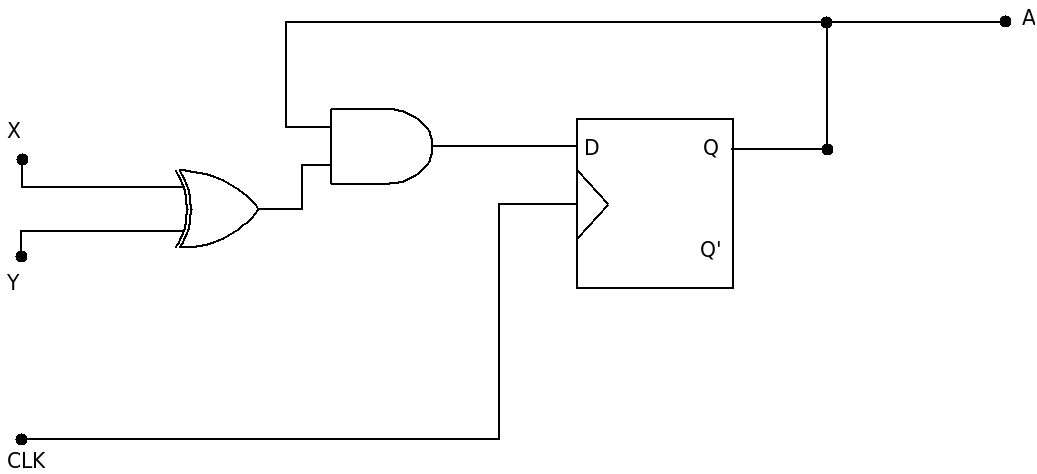
\includegraphics[width=0.5\textwidth]{FSM1}

Para esta máquina de estados, encuentre:
\begin{enumerate}
	\item La tabla de transición de estados.
	\item El diagrama de estados.
\end{enumerate}

\section*{Ejercicio 2}

Considere el siguiente diagrama lógico que describe una máquina de estados, con entradas \textit{X} y \textit{Y}, y salida \textit{A}.

\noindent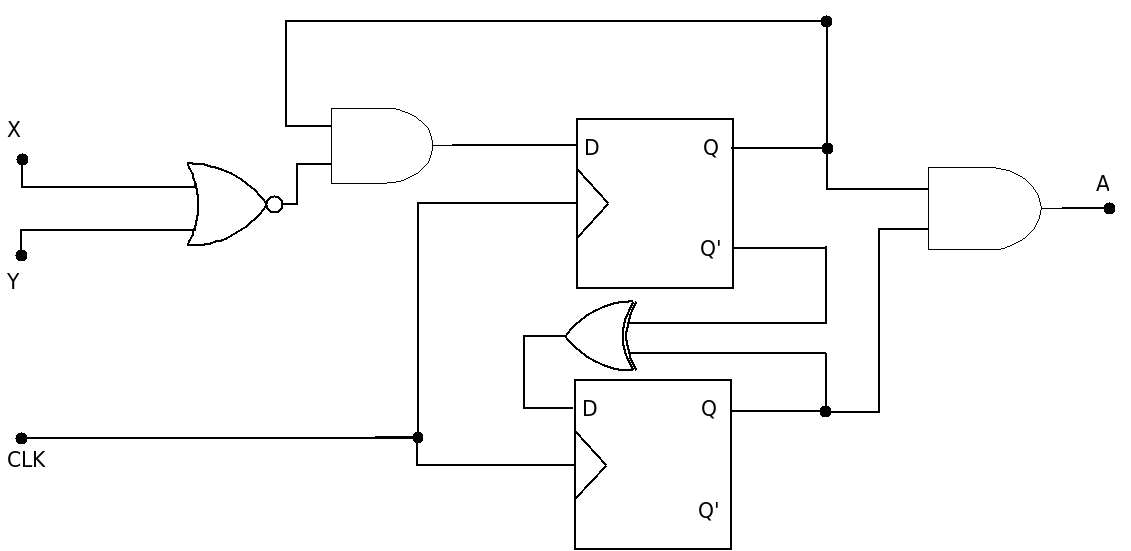
\includegraphics[width=0.5\textwidth]{FSM2}

Para esta máquina de estados, encuentre:
\begin{enumerate}
	\item La tabla de transición de estados.
	\item El diagrama de estados.
\end{enumerate}

\newpage

\section*{Ejercicio 3}

Considere el siguiente diagrama de estados para una máquina con una entrada \textit{X} y una salida \textit{B}.

\begin{center}
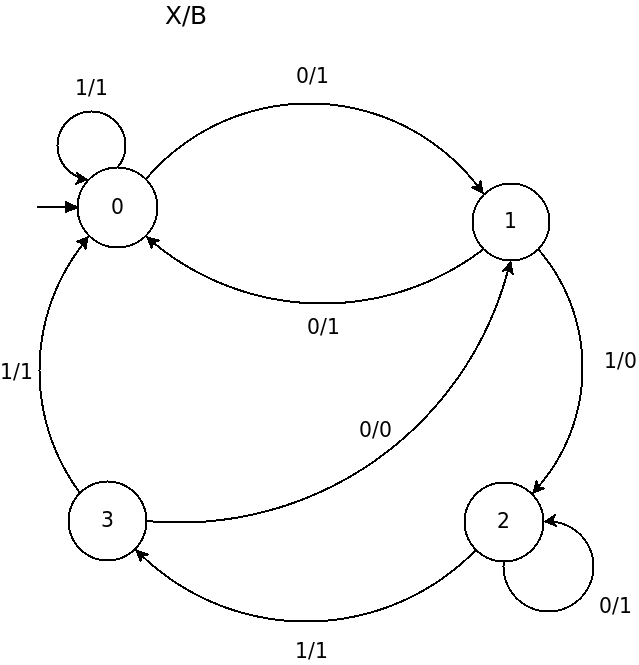
\includegraphics[width=0.3\textwidth]{FSM3}
\end{center}

Para esta diagrama de estados, encuentre:
\begin{enumerate}
	\item La tabla de transición de estados.
	\item El diagrama lógico para implementar la máquina de estados.
\end{enumerate}

\section*{Ejercicio 4}

Considere la siguiente tabla de transición de estados para una máquina con cuatro estados expresados por $S_B$ y $S_A$, una entrada $X$ y dos salidas $K$ y $L$.

\begin{center}
\begin{tabular}{cc|c|cc|cc}
\multicolumn{2}{c|}{Estado} & & \multicolumn{2}{c|}{Estado} & \multicolumn{2}{c}{}\\

\multicolumn{2}{c|}{Actual} & Entrada &
\multicolumn{2}{c|}{Próximo} & \multicolumn{2}{c}{Salidas}\\
 $S_B$ & $S_A$ & $X$ & $P_B$ & $P_A$ & $K$ & $L$ \\\hline
0 & 0 & 0 & 0 & 0 & 1 & 1 \\
0 & 0 & 1 & 1 & 1 & 1 & 1 \\
0 & 1 & 0 & 0 & 1 & 0 & 0 \\
0 & 1 & 1 & 1 & 0 & 0 & 0 \\
1 & 0 & 0 & 1 & 0 & 1 & 0 \\
1 & 0 & 1 & 0 & 0 & 1 & 0 \\
1 & 1 & 0 & 0 & 1 & 0 & 1 \\
1 & 1 & 1 & 1 & 1 & 0 & 1 \\
\end{tabular}
\end{center}

Con esta tabla, encuentre:
\begin{enumerate}
	\item El diagrama de estados.
	\item El diagrama lógico para implementar esta máquina de estados.
\end{enumerate}

\end{document}
